\documentclass[12pt,a4paper,french]{/home/nyaucki/Documents/Prof/CoursMaths/mycls/Exercices}

\begin{document}

\newcounter{chapter}
\setcounter{chapter}{1}
\title{\Roman{chapter} - Arithmétiques et durées}


\maketitle

%! TEX root = ../Exercices.tex
\section{Activités d'introductions}

\exo{IntroTrouverDiviseur} Pour introduire l'exercice type \textcolor{red}{todo}. A retravailler avec l'exercice \textcolor{red}{todo}.

On cherche à trouver tous les diviseurs de 12.

\begin{multicols}{3}
\foreach \x in {1,...,12}
	{
		\begin{itemize}[label={},leftmargin=0pt]
			\foreach \y in {quotient,reste}
			{\item Le \y~ de $12\div\x$~est : \filling[1cm]
			}
		\end{itemize}
}
\end{multicols}

Les diviseurs de 12 sont donc : \dotfill

\begin{enumerate}
	\item Etait-il nécessaire de faire la division pour vérifier si 1 était bien un diviseur ? \filling
	\item  Comment pouvait-on trouver les diviseurs supérieurs ou égaux à 4 sans faire de division ? 
		\dotlines{1}
	\item Si on souhaite aller le plus vite possible, les seules divisions à garder sont : \dotfill	
	\item Sur le cahier, chercher de la même manière tous les diviseurs de 28.
\end{enumerate}


\exo{IntroNombrePremier}

Cherchons si 79 est un nombre premier. Pour cela, cherhons les diviseurs de 79.

\begin{multicols}{3}
\foreach \x in {2,...,9}
	{
		\begin{itemize}[label={},leftmargin=0pt]
			\foreach \y in {quotient,reste}
			{\item Le \y~ de $79\div\x$~est : \filling[1cm]
			}
		\end{itemize}
}
\end{multicols}

Les diviseurs de 79 sont \fillin

\begin{enumerate}
	\item Pourquoi n'est-il pas nécessaire de continuer après 9 ?
		\dotlines{1}
	\item Comme 2 n'est pas diviseur de 79, pourquoi n'est-il pas nécessaire d'essayer avec 4 ? Quels-autres nombres nes sont pas nécessaires ?
		\dotlines{1}
	\item Au final, les seuls diviseurs qu'il est nécessaire de tester sont : \fillin.
	\item Sur le cahier, vérifier de la même manière si 83 est un nombre premier.
\end{enumerate}


\exo{IntroDecompositionNombrePremier}

Cherchons la décomposition en nombres premiers de 140.


On rappelle que les nombres premiers commencent par 2 ; 3 ; 5 ; 7 ; 11... et on va essayer de diviser 140 par ces nombres.
\begin{itemize}
	\item $140\div2=70$. On peut donc écrire $140=2 \times$\fillin
	\item $70\div2=35$. On peut donc écrire $140=2 \times$\fillin[1cm]$=2 \times2 \times$\fillin[1cm]
	\item \divreste{35}{3}. 3 n'entre donc pas dans la décomposition de 140.
	\item $35\div5=7$. On a donc $140=2 \times2 \times 5 \times$\fillin[1cm]
	\item 7 est un nombre premier, on ne peut donc pas aller plus loin.
\end{itemize}
La décomposition en produit de nombres premiers de 140 est donc :$140=$\dotfill.

\begin{enumerate}
	\item Donner la liste des nombres premiers inférieurs à 30 :
		\dotlines{1}
	\item Pourquoi n'avons nous pas essayer de diviser par 11 ?
		\dotlines{1}
	\item Sur le cahier, trouver de la même manière la décomposition de 132.
\end{enumerate}


\exo{IntroConversionDuree}

On cherche à convertir 12345 secondes en heures, minutes et secondes.

\begin{enumerate}
	\item Dans une minute, il y a \fillin secondes.
	\item je dois donc \fillin 12345 par 60 pour savoir combien il y a de minutes.
	\item On a : 12345 \fillin[0.5cm] 60 = \fillin[1cm] Reste \fillin[1cm].
	\item Dans une heure, il y a \fillin minutes.
	\item Je dois donc \fillin 205 par 60 pour savoir combien il y a d'heures.
	\item On a : 205 \fillin[0.5cm] 60 =\fillin[1cm] REste \fillin[1cm].
	\item Ainsi, 12345 secondes = \fillin[1cm] heures, \fillin[1cm] minutes et \fillin[1cm] secondes.
	\item Sur le cahier, de la même manière, convertire 9876 secondes en heures, minutes et secondes.
\end{enumerate}

On cherche maintenant à convertir 1,33 heures en secondes.

\begin{enumerate}
	\item Je dois \fillin par 60 pour savoir combien cela fait de minutes.
	\item On a : 1,33 \fillin[0.5cm] 60 = 79,8
	\item Je dois \fillin par 60 pour savoir combien cela fait de secondes.
	\item On a : 79,8 \fillin[0.5cm] 60 = \fillin.
	\item Ainsi, 1,33 heures = \fillin secondes.
	\item Sur le cahier, de la même manière, convertir 2,43 heures en secondes.
\end{enumerate}


\exo{IntroSommeDuree}

On cherche à ajouter 37 minutes à 14 heures et 45 minutes.

\begin{enumerate}
	\item Si on ne s'intéresse qu'on minutes, on doit faire la somme : 37+45=\fillin
	\item On peut convertir le résultat en heures et minutes, ce qui donne \fillin[1cm] heures et \fillin[1cm] minutes.
	\item On a donc :
		\begin{align*}
			14h45min+37min &= 14h + \fillin min\\
				       &= 14h + \fillin h + \fillin min\\
				       &= \fillin h + \fillin min
		\end{align*}
		
	\item Ainsi, en ajoutant 37 minutes à 14h45, on obtient \dotfill
	\item Sur le cahier, de la même manière, ajouter 28 secondes à 12 minutes et 46 secondes.
\end{enumerate}




%! TEX root = ../Exercices.tex
\section{Activités d'introductions}

\exo{Diviseur}
\begin{multicols}{3}
7 est il un diviseur de 155 ?
\dotlines{0}\columnbreak

8 est il un diviseur de 272 ?
\dotlines{0}\columnbreak

7 est il un diviseur de 231 ?
\dotlines{0}\columnbreak

\end{multicols}

\exo{TrouverDiviseur}Trouver tous les diviseurs des nombres suivants.
\begin{multicols}{3}
$$210$$
\dotlines{3}

$$140$$
\dotlines{3}\columnbreak

$$6$$
\dotlines{3}

$$2520$$
\dotlines{3}\columnbreak

$$60$$
\dotlines{3}

$$20$$
\dotlines{3}\columnbreak

\end{multicols}

\exo{Conversion}Convertir les durées suivantes en heures, mimnutes et secondes.
\begin{multicols}{3}
11053 s\dotfill

\vspace*{1em}\dotfill

9.86 h\dotfill

\vspace*{1em}\dotfill

22639 s\dotfill

\vspace*{1em}\dotfill

1.24 h\dotfill

\vspace*{1em}\dotfill\columnbreak

17227 s\dotfill

\vspace*{1em}\dotfill

6.54 h\dotfill

\vspace*{1em}\dotfill

14563 s\dotfill

\vspace*{1em}\dotfill

4.81 h\dotfill

\vspace*{1em}\dotfill\columnbreak

18716 s\dotfill

\vspace*{1em}\dotfill

6.03 h\dotfill

\vspace*{1em}\dotfill

6773 s\dotfill

\vspace*{1em}\dotfill

1.29 h\dotfill

\vspace*{1em}\dotfill\columnbreak

\end{multicols}

\exo{NombrePremier} : A faire sur le cahier. Les nombres suivants sont-ils premiers ?

\begin{multicols}{4}
	$$31$$

	$$51$$

	$$107$$

	$$97$$

	$$1028$$

	$$73$$

	$$91$$

	$$187$$

	$$111$$

	$$227$$

	$$341$$

	$$1001$$
\end{multicols}


\newpage

\exo{DecompositionNombrePremier}A faire sur le cahier. Décomposer les nombres suivants en poduit de nombres premiers.
\begin{multicols}{3}
$$4290$$

$$1540$$\columnbreak

$$39$$

$$2772$$\columnbreak

$$8190$$

$$429$$\columnbreak

\end{multicols}

\exo{AdditionnerDurees}A faire sur le cahier. Effectuer les opérations suivantes sur les durées
\begin{multicols}{3}
$$11\text{h }53\text{min }25\text{s }~+~2\text{h }30\text{min }54\text{s }$$

$$14\text{h }26\text{min }33\text{s }~-~2\text{h }42\text{min }55\text{s }\columnbreak$$

$$11\text{h }59\text{min }50\text{s }~+~7\text{h }38\text{min }54\text{s }$$

$$10\text{h }57\text{min }27\text{s }~-~2\text{h }44\text{min }34\text{s }\columnbreak$$

$$14\text{h }38\text{min }38\text{s }~+~4\text{h }26\text{min }37\text{s }$$

$$11\text{h }49\text{min }42\text{s }~-~9\text{h }40\text{min }57\text{s }\columnbreak$$

\end{multicols}




%! TEX root = ../Exercices.tex
\section{problèmes}

\exo{prop600}

601 est divisble par 1. 602 est divisible par 2. 603 est divisible par 3. Est-ce vrai pour tous les nombres entre 1 et 10 ?
\dotlines{1}

\exo{prop101}

1010 est un multiple de 10. 1111 est un multiple de 11. 1212 est un multiple de 12. Est-ce vrai pour tous les nombres entre 10 et 99 ?
\dotlines{1}

\exo{GOT7}

7 enfants on récupéré des bonbons pour Halloween et sont sur le point de se battre car il n'arrivent pas à partager.
\begin{itemize}
	\item Mark, qui ne veut pas se battre, préfère partir et abandonner sa part. Les 6 restants se rendent compte qu'ils peuvent alors partager équitablement.
	\item Jinyoung réalise que les bonbons sont au caramel et qu'il n'aime pas ça. Heureusement, les 5 restant peuvent encore partager équiteblement.
	\item Jackson est appelé par sa maman et doit rentrer tout de suite ! Le tas de bonbon peut encore être partagé entre les 4 restants.
	\item JB donne un bonbon à Jackson avant qu'il ne parte. Et c'est le drame, il n'est plus possible de partager équitablement en 4.
	\item Bambam recompte les bonbons et annonce que maintenant, il ne sera plus possible de faire de partage équitable.
\end{itemize}

\begin{enumerate}
	\item Quel type de nombre ne peut pas être partagé ? \dotfill
	\item Combien de bonbons y avait il au début ? \dotlines{2}
\end{enumerate}

\newpage

\exo{ExpliqueDecomposition}

\begin{enumerate}
	\item Quelle est la décomposition en produit de nombres premiers de 60 ?
		\dotlines{2}
	\item Donner tous les diviseurde de 60.
		\dotlines{2}
	\item Robin prétends qu'après avoir fait la décomposition en produit de nombres premiers, il est beaucoup plus facile de trouver tous les diviseurs d'un nombre. Pourquoi ?
		\dotlines{2}
	\item Sur le cahier, utiliser cette méthode pour trouver la liste des diviseurs de 72.
\end{enumerate}



\exo{PGCD1}

Un boulanger a préparé 90 croissants et 198 pains au chocolat. Il cherche à faire des lots équitables contenant tous le même nombre de croissants et le même nombre de pains au chocolat.

\begin{enumerate}
	\item Pourquoi ne peut-il pas faire 15 lots ? \dotfill
	\item Quelle est la décomposition produit de nombres premiers de 198 ?
		\dotlines{1}
	\item Donner tous les diviseurs de 90 et de 198.
		\dotlines{2}
	\item Combien de lots peut il faire au maximum? \dotfill
	\item Dans chaque lots, il y aura \fillin croissants et \fillin pains au chocolats.
\end{enumerate}

\exo{PGCD2}

C'est l'assault sur l'île d'Onigashima. Il y a 105 pirates et 140 samouraïs, et il serait judicieux de les répartir en groupe équitables.

\begin{enumerate}
	\item Pourquoi ne peut-on pas faire 21 groupes ? \dotfill
	\item Quelle est la décomposition produit de nombres premiers de 105 ?
		\dotlines{1}
	\item Donner tous les diviseurs de 140 et de 105.
		\dotlines{2}
	\item Combien de groupes peut-on faire au maximum? \dotfill
	\item Dans chaque groupe, il y aura \fillin pirates et \fillin samouraïs.
\end{enumerate}

\exo{Tarot}

Un jeu de tarot contient 78 cartes comprenant 21 atouts, une carte appelée "Excuse" et les cartes restantes sont partagées en 4 couleurs : coeur, carreau, pique et trèfle.

\begin{enumerate}
	\item Combien de carte y a-t-il par couleur ?
		\dotlines{1}

		Le tarot peut se jouer à 3, 4 ou 5. On distribue équitablement les cartes aux joueurs, et ce qui reste est appelé "le chien" et est donné au joueur qui attaque.  
\item Remplir le tableau suivant :
		\begin{tabular}{c*{3}{|c}}
			\renewcommand{\arraystretch}{3.5}
			Nombre de joueurs & 3 & 4 & 5 \\\hline&&&\\[0.5cm]
			Cartes par joueurs & \fillin[1cm] & 18 & 15 \\\hline&&&\\[0.5cm]
			Cartes dans le chien & 6 & \fillin[1cm] & \fillin[1cm]\\[0.1cm] &&&
		\end{tabular}

	\item Lenon dit " Dans tous les cas, le chien est trop gros. On pourrait mettre moins de carte dans le chien et en donner plus au joueurs". A-t-il raison ? Pourquoi ?
		\dotlines{2}
	\item John a perdu 3 cartes dans son jeu, mais veut malgré tout joueur. Il voudrait savoir combien de cartes ditribuer à chaque personne pour que le nombre de carte dans le chien soit le plus proche possible de ce qui est distribué avec un jeu complet :

		\begin{tabular}{c*{3}{|c}}
			\renewcommand{\arraystretch}{3.5}
			Nombre de joueurs & 3 & 4 & 5 \\\hline&&&\\[0.5cm]
			Cartes par joueurs & \fillin[1cm] & \fillin[1cm]& \fillin[1cm]\\\hline&&&\\[0.5cm]
			Cartes dans le chien & \fillin[1cm] & \fillin[1cm] & \fillin[1cm]\\[0.1cm] &&&
		\end{tabular}
	\item Même question, mais pour Bob qui possède un jeu où il manque 4 cartes.

		\begin{tabular}{c*{3}{|c}}
			\renewcommand{\arraystretch}{3.5}
			Nombre de joueurs & 3 & 4 & 5 \\\hline&&&\\[0.5cm]
			Cartes par joueurs & \fillin[1cm] & \fillin[1cm]& \fillin[1cm]\\\hline&&&\\[0.5cm]
			Cartes dans le chien & \fillin[1cm] & \fillin[1cm] & \fillin[1cm]\\[0.1cm] &&&
		\end{tabular}
\end{enumerate}

\newpage

\exo{Celimene}

Pour l'anniversaire de Célimène, ses parents ont préparé 27 fondants au chocolats. Célimène va les partager équitablement avec ses copines, puis comme c'est son anniversaire, elle pourra aussi avoir les fondant restants.

\begin{enumerate}
	\item Si elle invite 4 copines, combien de fondants aura Célimène ?
		\dotlines{1}
	\item Si elle invite 6 copines, combien de fondants aura Célimène ?
		\dotlines{1}
	\item Vaut-il mieux pour Célimène inviter 4 ou 6 copines ?\dotfill
	\item Célimène doit inviter entre 2 et 10 copines. Quel est le nombre de copine qui lui permettra d'avoir le plus de fondants possible ?
		\dotlines{3}
\end{enumerate}

\exo{Impression}

L'imprimante du collège met 3 secondes pour imprimmer 1 page. Monsieur Loizon veut imprimmer un document de 5 pages pour chacun de ses 76 élèves de 5ème. La récrée dure 15 minutes, aura-t-il assez de temps ? 
\dotlines{3}


\section{Exercices ludiques}

\exo{pyramide} Compléter les pyramides suivantes de sorte à ce que chaque case soit égale à la somme des deux cases du dessous. Ecrire les résultats en heures, minutes et secondes.

\begin{minipage}[t]{0.45\textwidth}
	\begin{center}
	\begin{tikzpicture}[scale=1.05]
 		\foreach \j [count=\xi]  in { }
 				{\draw (-3+2*\xi,0) rectangle (-1+2*\xi,1);
 				\node at (-2+2*\xi,0.5) {\j};}
 		\foreach \j [count=\xi]  in { ,  }
 				{\draw (-4+2*\xi,-1) rectangle (-2+2*\xi,0);
 				\node at (-3+2*\xi,-0.5) {\j};}
 		\foreach \j [count=\xi]  in { ,  , 2min 05s}
 				{\draw (-5+2*\xi,-2) rectangle (-3+2*\xi,-1);
 				\node at (-4+2*\xi,-1.5) {\j};}
 		\foreach \j [count=\xi]  in {1min 22s, 41s, 37s, }
 				{\draw (-6+2*\xi,-3) rectangle (-4+2*\xi,-2);
 				\node at (-5+2*\xi,-2.5) {\j};}
\end{tikzpicture}
	\end{center}

\end{minipage}
\hfil
\vrule
\hfil
\begin{minipage}[t]{0.45\textwidth}
	\begin{center}
	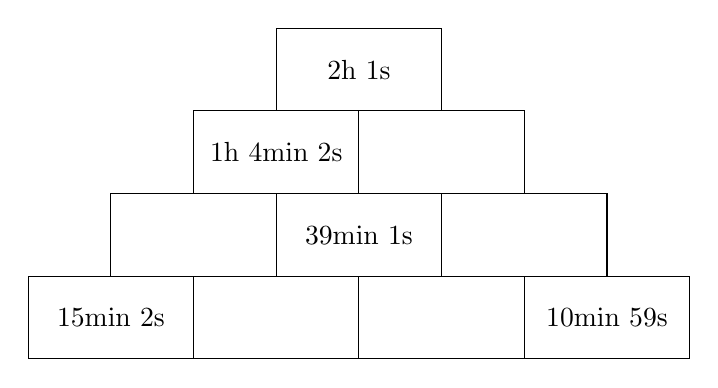
\begin{tikzpicture}[scale=1.05]
 		\foreach \j [count=\xi]  in {2h 1s}
 				{\draw (-3+2*\xi,0) rectangle (-1+2*\xi,1);
 				\node at (-2+2*\xi,0.5) {\j};}
 		\foreach \j [count=\xi]  in {1h 4min 2s,  }
 				{\draw (-4+2*\xi,-1) rectangle (-2+2*\xi,0);
 				\node at (-3+2*\xi,-0.5) {\j};}
 		\foreach \j [count=\xi]  in { , 39min 1s,  }
 				{\draw (-5+2*\xi,-2) rectangle (-3+2*\xi,-1);
 				\node at (-4+2*\xi,-1.5) {\j};}
 		\foreach \j [count=\xi]  in {15min 2s,  ,  , 10min 59s}
 				{\draw (-6+2*\xi,-3) rectangle (-4+2*\xi,-2);
 				\node at (-5+2*\xi,-2.5) {\j};}
\end{tikzpicture}
	\end{center}

\end{minipage}

\newpage 

\exo{sudoku} Compléter les grilles de Sudoku suivantes en inscrivant les restes des divisions euclidiennes dans les cases données, puis à l'aide des règles classiques de Sudoku.
\vfil
\setlength{\columnseprule}{0pt}\begin{minipage}{0.55\textwidth}
\begin{center}
	 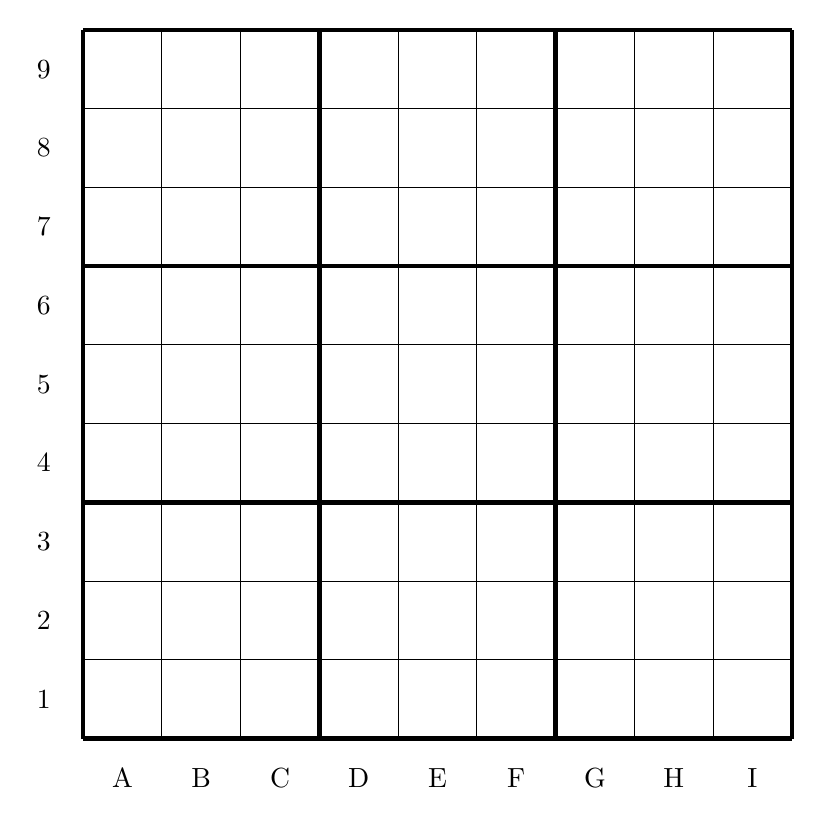
\begin{tikzpicture}
		 \draw[thin] (0,0) grid (9,9);
		 \draw[ultra thick,step=3] (0,0) grid (9,9);
		 \foreach \x/\y in {1/A,2/B,3/C,4/D,5/E,6/F,7/G,8/H,9/I}
			 { \draw node at (\x-0.5,-0.5) {\y};
			 \draw node at (-0.5,\x-0.5) {\x}; }
		 \end{tikzpicture}	
	 \end{center}
\end{minipage}
\hfil\vrule\hfil
\begin{minipage}{0.4\textwidth}
\begin{itemize}[leftmargin=10pt]\begin{multicols}{2}
\item(A;9) : 90852\div11

\item(C;9) : 9973\div4

\item(E;9) : 92801\div11

\item(G;9) : 77785\div9

\item(I;9) : 36210\div11

\item(B;8) : 20999\div5

\item(D;8) : 27668\div11

\item(F;8) : 17015\div11

\item(H;8) : 61485\div11

\item(A;7) : 5815\div8

\item(C;7) : 29049\div10

\item(E;7) : 65092\div7

\item(G;7) : 26218\div5

\item(I;7) : 42106\div6

\item(B;6) : 797\div6

\item(H;6) : 34432\div6

\item(A;5) : 64316\div10

\item(C;5) : 9573\div11

\item(E;5) : 36412\div6

\item(G;5) : 34659\div10

\item(I;5) : 23115\div7

\item(B;4) : 29140\div11

\item(H;4) : 2399\div8

\item(A;3) : 17225\div7

\item(C;3) : 24972\div8

\item(E;3) : 13105\div9

\item(G;3) : 48487\div5

\item(I;3) : 17056\div11

\item(B;2) : 39697\div11

\item(D;2) : 32734\div6

\item(F;2) : 78438\div8

\item(H;2) : 14640\div7

\item(A;1) : 57690\div8

\item(C;1) : 106794\div11

\item(E;1) : 74330\div9

\item(G;1) : 27472\div6

\item(I;1) : 37583\div8

\item[\vspace{\fill}]\end{multicols}\end{itemize}\end{minipage}
\vfil
\setlength{\columnseprule}{0pt}\begin{minipage}{0.55\textwidth}
\begin{center}
	 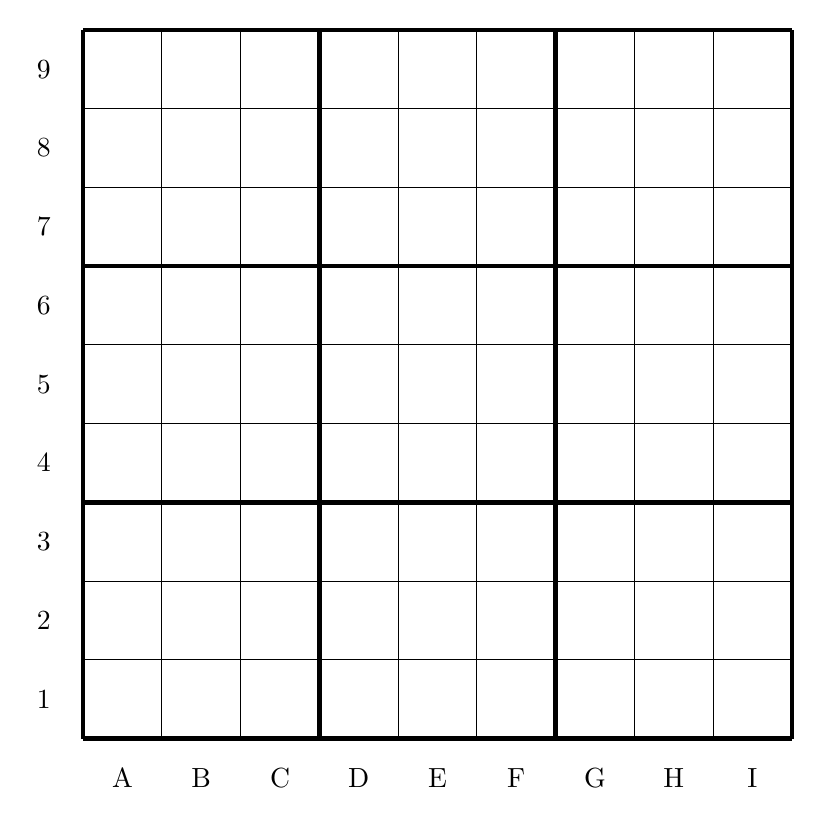
\begin{tikzpicture}
		 \draw[thin] (0,0) grid (9,9);
		 \draw[ultra thick,step=3] (0,0) grid (9,9);
		 \foreach \x/\y in {1/A,2/B,3/C,4/D,5/E,6/F,7/G,8/H,9/I}
			 { \draw node at (\x-0.5,-0.5) {\y};
			 \draw node at (-0.5,\x-0.5) {\x}; }
		 \end{tikzpicture}	
	 \end{center}
\end{minipage}
\hfil\vrule\hfil
\begin{minipage}{0.4\textwidth}
\begin{itemize}[leftmargin=10pt]\begin{multicols}{2}
\item(A;9) : 5233\div11

\item(E;9) : 54031\div7

\item(I;9) : 89950\div9

\item(B;8) : 41073\div6

\item(D;8) : 29901\div7

\item(E;8) : 19680\div11

\item(F;8) : 52442\div10

\item(H;8) : 2556\div15

\item(C;7) : 104077\div15

\item(G;7) : 55172\div18

\item(D;6) : 143271\div18

\item(A;5) : 8518\div8

\item(B;5) : 57704\div10

\item(E;5) : 144316\div17

\item(H;5) : 66239\div7

\item(I;5) : 128067\div14

\item(F;4) : 40497\div8

\item(C;3) : 152172\div17

\item(G;3) : 155891\div16

\item(B;2) : 179197\div19

\item(D;2) : 115441\div13

\item(E;2) : 15562\div17

\item(F;2) : 8572\div13

\item(H;2) : 14185\div16

\item(A;1) : 79583\div11

\item(E;1) : 139998\div19

\item(I;1) : 50531\div11

\item[\vspace{\fill}]\end{multicols}\end{itemize}\end{minipage}

\newpage
\input{Exercices_Contenu/PixelArt1.tex}

\exo{Labyrinthe1} Traverser le labyrinthe en franchissant les cases dans l'ordre croissant 

\begin{center}
\tikzmath{\sizex = 7 ;\sizexm=\sizex-1 ; \sizey=7 ; \sizeym=\sizey-1;}
\begin{tikzpicture}[scale=1.5]
	\foreach \i in {0,...,\sizex}
 		{\foreach \j in {0,...,\sizey}
 			{\draw ({max(\i-0.2,0)},\j)--({min(\sizex,\i+0.2)},\j);
			\draw (\i,{max(0,\j-0.2)})--(\i,{min(\sizey,\j+0.2)}); }}
	\draw (0,0) rectangle (\sizex,\sizey) ;
	\draw[thick,white] (0,\sizey-0.1)--(0,\sizeym+0.2) ;
 	\draw[thick,white] (\sizex,0.2)--(\sizex,0.8) ;
	\draw[-{Latex[length=3mm,width=5mm]}] (-0.5,\sizey-0.5)--(0,\sizey-0.5) ;
	\draw[-{Latex[length=3mm,width=5mm]}] (\sizex,0.5)--(\sizex+0.5,0.5) ;
	\node at (0.5,6.5) {92s};
	\node at (1.5,6.5) {1.23min};
	\node at (2.5,6.5) {245s};
	\node at (3.5,6.5) {3.95min};
	\node at (4.5,6.5) {272s};
	\node at (5.5,6.5) {4.81min};
	\node at (6.5,6.5) {291s};
	\node at (0.5,5.5) {1.56min};
	\node at (1.5,5.5) {74s};
	\node at (2.5,5.5) {4.16min};
	\node at (3.5,5.5) {259s};
	\node at (4.5,5.5) {4.4min};
	\node at (5.5,5.5) {248s};
	\node at (6.5,5.5) {5.18min};
	\node at (0.5,4.5) {98s};
	\node at (1.5,4.5) {1.48min};
	\node at (2.5,4.5) {238s};
	\node at (3.5,4.5) {3.76min};
	\node at (4.5,4.5) {262s};
	\node at (5.5,4.5) {5.6min};
	\node at (6.5,4.5) {323s};
	\node at (0.5,3.5) {2.0min};
	\node at (1.5,3.5) {100s};
	\node at (2.5,3.5) {3.93min};
	\node at (3.5,3.5) {228s};
	\node at (4.5,3.5) {3.45min};
	\node at (5.5,3.5) {350s};
	\node at (6.5,3.5) {5.21min};
	\node at (0.5,2.5) {137s};
	\node at (1.5,2.5) {2.63min};
	\node at (2.5,2.5) {142s};
	\node at (3.5,2.5) {3.76min};
	\node at (4.5,2.5) {216s};
	\node at (5.5,2.5) {6.1min};
	\node at (6.5,2.5) {347s};
	\node at (0.5,1.5) {1.9min};
	\node at (1.5,1.5) {176s};
	\node at (2.5,1.5) {3.3min};
	\node at (3.5,1.5) {204s};
	\node at (4.5,1.5) {3.03min};
	\node at (5.5,1.5) {380s};
	\node at (6.5,1.5) {6.7min};
	\node at (0.5,0.5) {93s};
	\node at (1.5,0.5) {2.55min};
	\node at (2.5,0.5) {187s};
	\node at (3.5,0.5) {3.06min};
	\node at (4.5,0.5) {177s};
	\node at (5.5,0.5) {6.13min};
	\node at (6.5,0.5) {412s};
\end{tikzpicture}
\end{center}

\newpage
\exo{PixelArt2}Colorie en noir uniquement les nombres qui ne sont pas premiers.

\begin{figure}[H]
\center
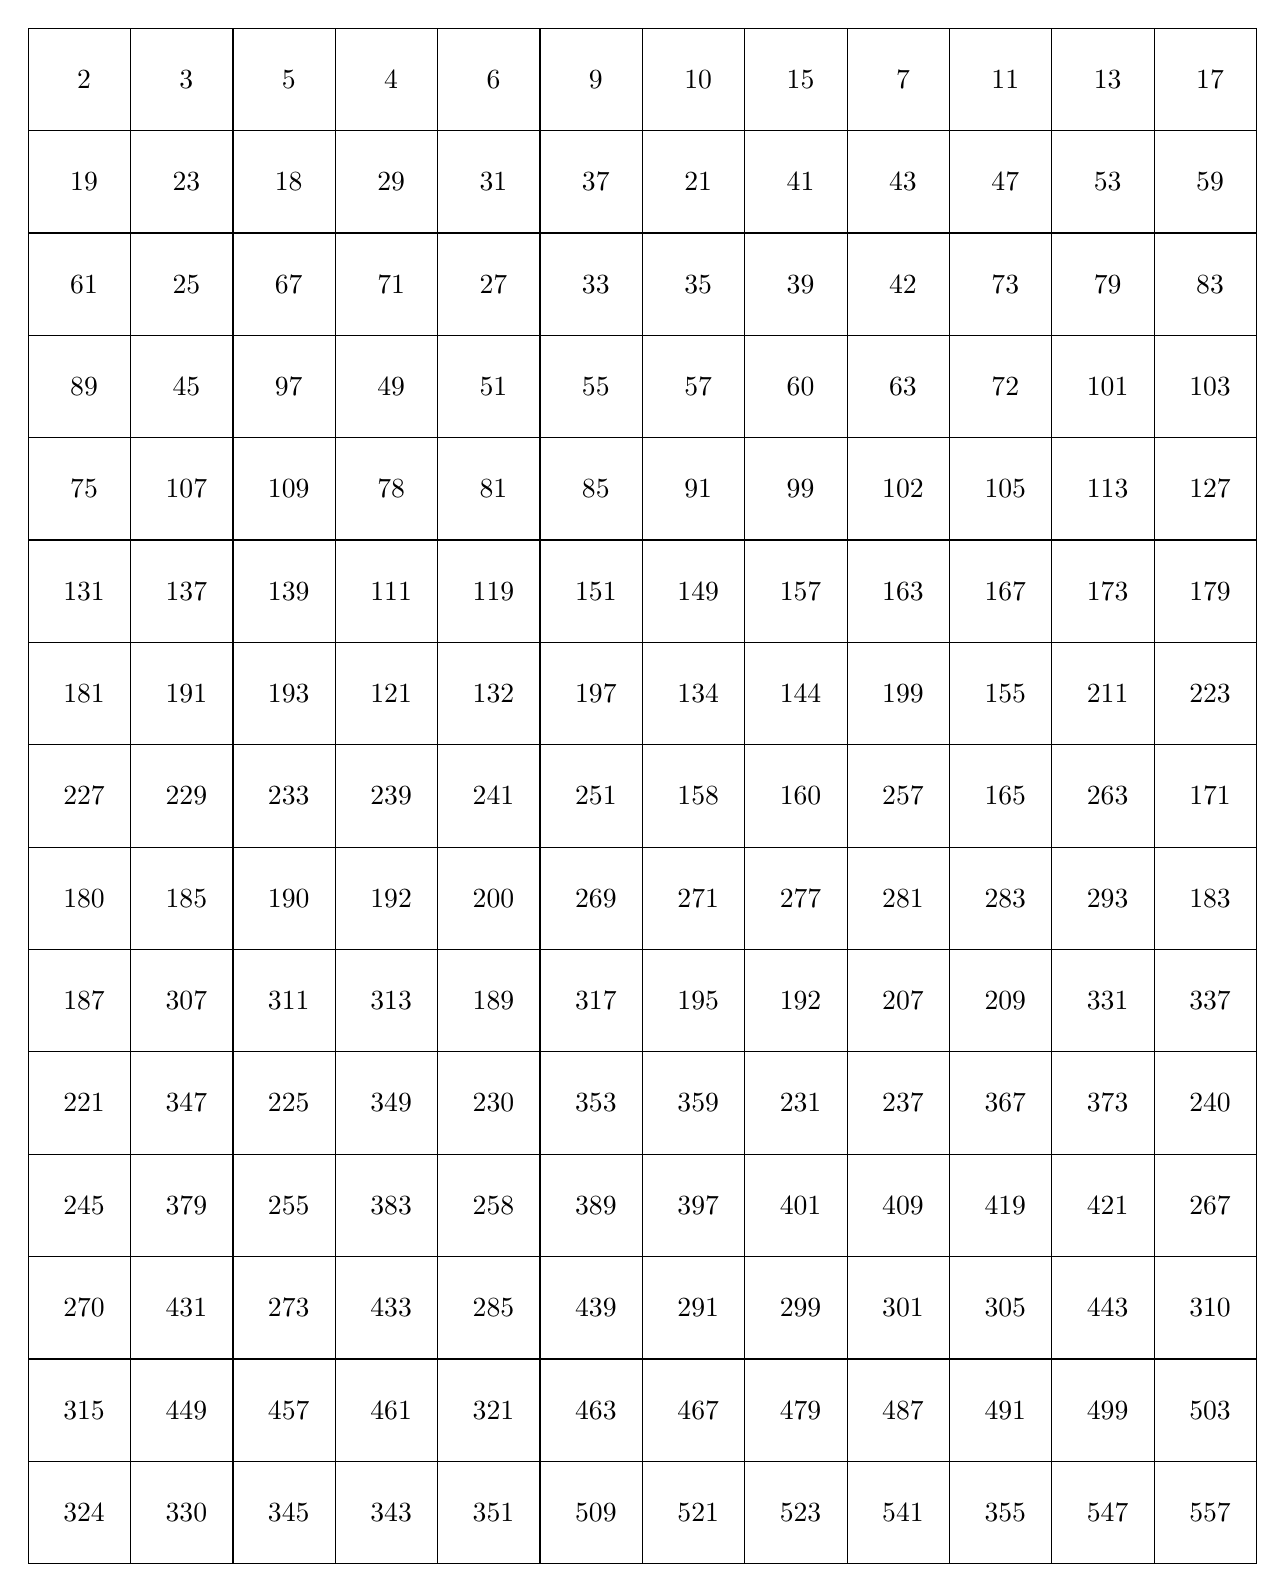
\begin{tikzpicture}[scale=1.3]
\newcommand{\y}{0}\renewcommand{\y}{0}
\foreach \x [count=\xi] in {2, 3, 5, 4, 6, 9, 10, 15, 7, 11, 13, 17}
{\draw (\xi,\y) rectangle (\xi +1,\y -1) node[pos=0.5]{{ \x}};}
\renewcommand{\y}{-1}
\foreach \x [count=\xi] in {19, 23, 18, 29, 31, 37, 21, 41, 43, 47, 53, 59}
{\draw (\xi,\y) rectangle (\xi +1,\y -1) node[pos=0.5]{{ \x}};}
\renewcommand{\y}{-2}
\foreach \x [count=\xi] in {61, 25, 67, 71, 27, 33, 35, 39, 42, 73, 79, 83}
{\draw (\xi,\y) rectangle (\xi +1,\y -1) node[pos=0.5]{{ \x}};}
\renewcommand{\y}{-3}
\foreach \x [count=\xi] in {89, 45, 97, 49, 51, 55, 57, 60, 63, 72, 101, 103}
{\draw (\xi,\y) rectangle (\xi +1,\y -1) node[pos=0.5]{{ \x}};}
\renewcommand{\y}{-4}
\foreach \x [count=\xi] in {75, 107, 109, 78, 81, 85, 91, 99, 102, 105, 113, 127}
{\draw (\xi,\y) rectangle (\xi +1,\y -1) node[pos=0.5]{{ \x}};}
\renewcommand{\y}{-5}
\foreach \x [count=\xi] in {131, 137, 139, 111, 119, 151, 149, 157, 163, 167, 173, 179}
{\draw (\xi,\y) rectangle (\xi +1,\y -1) node[pos=0.5]{{ \x}};}
\renewcommand{\y}{-6}
\foreach \x [count=\xi] in {181, 191, 193, 121, 132, 197, 134, 144, 199, 155, 211, 223}
{\draw (\xi,\y) rectangle (\xi +1,\y -1) node[pos=0.5]{{ \x}};}
\renewcommand{\y}{-7}
\foreach \x [count=\xi] in {227, 229, 233, 239, 241, 251, 158, 160, 257, 165, 263, 171}
{\draw (\xi,\y) rectangle (\xi +1,\y -1) node[pos=0.5]{{ \x}};}
\renewcommand{\y}{-8}
\foreach \x [count=\xi] in {180, 185, 190, 192, 200, 269, 271, 277, 281, 283, 293, 183}
{\draw (\xi,\y) rectangle (\xi +1,\y -1) node[pos=0.5]{{ \x}};}
\renewcommand{\y}{-9}
\foreach \x [count=\xi] in {187, 307, 311, 313, 189, 317, 195, 192, 207, 209, 331, 337}
{\draw (\xi,\y) rectangle (\xi +1,\y -1) node[pos=0.5]{{ \x}};}
\renewcommand{\y}{-10}
\foreach \x [count=\xi] in {221, 347, 225, 349, 230, 353, 359, 231, 237, 367, 373, 240}
{\draw (\xi,\y) rectangle (\xi +1,\y -1) node[pos=0.5]{{ \x}};}
\renewcommand{\y}{-11}
\foreach \x [count=\xi] in {245, 379, 255, 383, 258, 389, 397, 401, 409, 419, 421, 267}
{\draw (\xi,\y) rectangle (\xi +1,\y -1) node[pos=0.5]{{ \x}};}
\renewcommand{\y}{-12}
\foreach \x [count=\xi] in {270, 431, 273, 433, 285, 439, 291, 299, 301, 305, 443, 310}
{\draw (\xi,\y) rectangle (\xi +1,\y -1) node[pos=0.5]{{ \x}};}
\renewcommand{\y}{-13}
\foreach \x [count=\xi] in {315, 449, 457, 461, 321, 463, 467, 479, 487, 491, 499, 503}
{\draw (\xi,\y) rectangle (\xi +1,\y -1) node[pos=0.5]{{ \x}};}
\renewcommand{\y}{-14}
\foreach \x [count=\xi] in {324, 330, 345, 343, 351, 509, 521, 523, 541, 355, 547, 557}
{\draw (\xi,\y) rectangle (\xi +1,\y -1) node[pos=0.5]{{ \x}};}
\end{tikzpicture}
\end{figure}

\newpage
\exo{Labyrinthe2} Traverser le labyrinthe en franchissant les cases dans l'ordre décroissant 

\begin{center}
\tikzmath{\sizex = 9 ;\sizexm=\sizex-1 ; \sizey=10 ; \sizeym=\sizey-1;}
\begin{tikzpicture}[scale=1.7]
	\foreach \i in {0,...,\sizex}
 		{\foreach \j in {0,...,\sizey}
 			{\draw ({max(\i-0.2,0)},\j)--({min(\sizex,\i+0.2)},\j);
			\draw (\i,{max(0,\j-0.2)})--(\i,{min(\sizey,\j+0.2)}); }}
	\draw (0,0) rectangle (\sizex,\sizey) ;
	\draw[thick,white] (0,\sizey-0.1)--(0,\sizeym+0.2) ;
 	\draw[thick,white] (\sizex,0.2)--(\sizex,0.8) ;
	\draw[-{Latex[length=3mm,width=5mm]}] (-0.5,\sizey-0.5)--(0,\sizey-0.5) ;
	\draw[-{Latex[length=3mm,width=5mm]}] (\sizex,0.5)--(\sizex+0.5,0.5) ;
	\node at (0.5,9.5) {2392s};
	\node at (1.5,9.5) {39.53min};
	\node at (2.5,9.5) {2352s};
	\node at (3.5,9.5) {39.06min};
	\node at (4.5,9.5) {2025s};
	\node at (5.5,9.5) {33.38min};
	\node at (6.5,9.5) {1991s};
	\node at (7.5,9.5) {33.18min};
	\node at (8.5,9.5) {2004s};
	\node at (0.5,8.5) {39.65min};
	\node at (1.5,8.5) {2370s};
	\node at (2.5,8.5) {38.85min};
	\node at (3.5,8.5) {2319s};
	\node at (4.5,8.5) {33.8min};
	\node at (5.5,8.5) {2022s};
	\node at (6.5,8.5) {33.33min};
	\node at (7.5,8.5) {1996s};
	\node at (8.5,8.5) {33.08min};
	\node at (0.5,7.5) {2309s};
	\node at (1.5,7.5) {38.75min};
	\node at (2.5,7.5) {2328s};
	\node at (3.5,7.5) {38.73min};
	\node at (4.5,7.5) {2032s};
	\node at (5.5,7.5) {33.48min};
	\node at (6.5,7.5) {1980s};
	\node at (7.5,7.5) {32.9min};
	\node at (8.5,7.5) {1963s};
	\node at (0.5,6.5) {38.51min};
	\node at (1.5,6.5) {2320s};
	\node at (2.5,6.5) {38.61min};
	\node at (3.5,6.5) {2064s};
	\node at (4.5,6.5) {34.03min};
	\node at (5.5,6.5) {2036s};
	\node at (6.5,6.5) {32.51min};
	\node at (7.5,6.5) {1967s};
	\node at (8.5,6.5) {32.55min};
	\node at (0.5,5.5) {2291s};
	\node at (1.5,5.5) {38.58min};
	\node at (2.5,5.5) {2069s};
	\node at (3.5,5.5) {34.76min};
	\node at (4.5,5.5) {2063s};
	\node at (5.5,5.5) {34.65min};
	\node at (6.5,5.5) {1880s};
	\node at (7.5,5.5) {32.45min};
	\node at (8.5,5.5) {1939s};
	\node at (0.5,4.5) {37.98min};
	\node at (1.5,4.5) {2272s};
	\node at (2.5,4.5) {37.68min};
	\node at (3.5,4.5) {2107s};
	\node at (4.5,4.5) {35.25min};
	\node at (5.5,4.5) {1882s};
	\node at (6.5,4.5) {31.55min};
	\node at (7.5,4.5) {1904s};
	\node at (8.5,4.5) {32.05min};
	\node at (0.5,3.5) {2257s};
	\node at (1.5,3.5) {37.68min};
	\node at (2.5,3.5) {2250s};
	\node at (3.5,3.5) {35.16min};
	\node at (4.5,3.5) {2124s};
	\node at (5.5,3.5) {35.25min};
	\node at (6.5,3.5) {1883s};
	\node at (7.5,3.5) {31.48min};
	\node at (8.5,3.5) {1907s};
	\node at (0.5,2.5) {37.45min};
	\node at (1.5,2.5) {2258s};
	\node at (2.5,2.5) {37.58min};
	\node at (3.5,2.5) {2153s};
	\node at (4.5,2.5) {35.7min};
	\node at (5.5,2.5) {2138s};
	\node at (6.5,2.5) {31.11min};
	\node at (7.5,2.5) {1865s};
	\node at (8.5,2.5) {30.76min};
	\node at (0.5,1.5) {2237s};
	\node at (1.5,1.5) {37.53min};
	\node at (2.5,1.5) {2172s};
	\node at (3.5,1.5) {36.06min};
	\node at (4.5,1.5) {2146s};
	\node at (5.5,1.5) {35.65min};
	\node at (6.5,1.5) {1856s};
	\node at (7.5,1.5) {30.93min};
	\node at (8.5,1.5) {1850s};
	\node at (0.5,0.5) {37.11min};
	\node at (1.5,0.5) {2204s};
	\node at (2.5,0.5) {36.36min};
	\node at (3.5,0.5) {2175s};
	\node at (4.5,0.5) {35.5min};
	\node at (5.5,0.5) {2144s};
	\node at (6.5,0.5) {30.51min};
	\node at (7.5,0.5) {1842s};
	\node at (8.5,0.5) {30.5min};
\end{tikzpicture}
\end{center}




\section{Pour aller plus loin}
\exo{AlgoEuclide}
\begin{enumerate}
	\item Chercher ce qu'est un PGCD.
	\item Chercher ce qu'est l'algorithme d'Euclide et comment il fonctionne.
	\item Utiliser l'algorithme d'Euclide pour déterminer le PGCD de 2048 et 7544.
	\item Réaliser une affiche pour présenter l'algorithme d'Euclide à vos camarades.
\end{enumerate}


\end{document}
